\documentclass[a4paper,12pt]{article}
\usepackage[utf8]{inputenc}
\usepackage[english]{babel}
\usepackage{authblk}
\usepackage{graphicx}
\usepackage{mathptmx}
\usepackage[singlespacing]{setspace}
\usepackage[headheight=1in,margin=1in]{geometry}
\usepackage{fancyhdr}
\usepackage{lipsum}


\renewcommand{\headrulewidth}{0pt}
\pagestyle{fancy}

\usepackage{natbib}
\bibliographystyle{abbrvnat}
\setcitestyle{authoryear} 



\makeatletter
\def\@maketitle{%
  \newpage

  \begin{center}%
  \let \footnote \thanks
    {\LARGE \@title \par}%
  \end{center}%
  \par
  \vskip 0.1em}
\makeatother

\chead{%
  $9$$^{th}$ International Conference on Computational Social Science IC$^{2}$S$^{2}$\\
  July 17-20, 2023, Copenhagen, Denmark%
}

\title{Development of Educational Segregation Measured using Longitudinal Population Scale Network Data}

 
\date{}

\begin{document}

\maketitle
\thispagestyle{fancy}

\begin{center}
\textit{Keywords: network analysis, segregation, complete population, longitudinal, education level}
\newline
\end{center}

\section*{Extended Abstract}

\paragraph{Introduction}
 Segregation is an important social issue and an enduring theme for policy makers. Educational segregation can promote 'social bubbles', reinforce societal polarisation processes and lead to lower social cohesion \citep{Blossfeld2010,Iyengar2019}. Furthermore, if the lower educated have a limited number of contacts outside their own group, this may lead to increasing opportunity inequality: a larger, more mixed network can be an important form of social capital on the labour market, especially the so-called weak ties \citep{Granovetter1973}. Segregation is in essence a network problem since it addresses the question to what extent  people from different groups are connected to each other either directly or indirectly. Using network data covering the entire population of the Netherlands \citep{Laan2022}, we investigate how educational segregation changed over time, as well as studying age-specific patterns.

\paragraph{Data}
Statistics Netherlands derived a population scale network for the entire Dutch population \citep{Laan2022}. This network is derived from official administrative government registers \citep{Bakker2014} and includes family members, household members, colleagues, class mates and neighbours at multiple times points, from January 1st 2009 yearly up until January 1st 2020. Using these longitudinal networks it is possible to look at how the educational segregation and the development of the segregation changes in this period. We will focus on the ages 25 to 55 years old. The lower bound based on the fact that around that age most people will have reached their final education level. The upper bound is based on the fact that information on education level becomes more incomplete after this age. In the analyses below we use data from 2013 up until 2020. In 2013 there has been a change in the data on education level. This introduces unreliable estimates of change for specific age groups and education levels.

\paragraph{Methods}
We largely follow the methods as used by \cite{Laan2022}. First, we removed the family relations between household members only keeping the household relations. Second, weights were determined for each relation for each ego: the relations for each layer (family, household, work, neighbourhood and school) were given an equal total weight. This ensures that each layer is equally important in the network. Third, each ego is given a weight. Persons with a known education level have a weight larger than zero (to correct for missing values in education level). Persons younger than 25 and older than 55 are given a weight equal to 0. Note that these persons are kept in the network and, therefore, through them other parts of the network can be reached although they don't contribute directly to the measured segregation of the target population . Finally, a localised random walk (localised page rank) was performed for each person in the network \citep{Ballester2014}. This results in an exposure score for each person to each of the four education levels. The exposure of a person to their own education level ($e_i$) compared to the expected exposure for that education level ($E_i$) is a measure of segregation (corresponds to \textit{V} from \cite{Massey1988}):
% Oud stuk zin: their connections contribute to the measured segregation of our target population
\begin{equation}
  s_i = \frac{e_i - E_i}{1 - E_i}.
\end{equation}
$E_i$ is determined by the weighed (by distance using a tri-cube weight function) fraction of persons with the given education level in a radius of 30 kilometre. The result is a segregation score for each individual in each of the 11 years. These individual scores can be aggregated to age, education level, etc. Furthermore, by linking the results from different years, it is possible to measure how, at an individual level, the segregation score has changed. 

\paragraph{Results}
Figure~\ref{fig:lft} shows the mean segregation score as a function of age, education level and year. The segregation is highest for the lower and master educated. Generally, the segregation increases until the age of 30--35 after which it stays stable for a number of years. For bachelor and master educated the segregation increases further after 45-50 years. This seems to be a cohort effect of persons born before 1970 as this effect shifts by a year each year.  

In order to look purely at the age effects, the individual segregation in year \textit{t} can be compared to that in year \textit{t}+1. Figure~\ref{fig:cor} shows the correlation between segregation in two sequential years. The differences between the different years are small. Only 2019 for intermediate level educated seems to differ somewhat. This could be caused by the COVID-19 pandemic in 2020 which could have affected the work network in 2020 (this is also visible in the next figure). In general segregation is strongly correlated in time. The correlation is lower at younger ages. In this period the networks of persons show more changes: persons are moving address more often, they are finding partners and developing their careers. 

Figure~\ref{fig:ontw} shows the average change in individual segregation from year \textit{t} to year \textit{t}+1. For most education levels the segregation increases in the ages from 25 to approximately 30. After that the segregation decreases slowly. In general the differences between the different years are small. Only for the lower educated, the variation is larger where in more recent years the decrease in segregation seems to be somewhat smaller. It should also be noted that the year-on-year change in segregation is small relative to the overall differences in segregation between the different education levels. Therefore, the segregation one has around the age of 30 for a large part determines the segregation at later ages.

\paragraph{Conclusion} 
Using the longitudinal networks, it is possible to measure the segregation of persons with respect to education level for different time periods in a persons life. This makes it possible to study the effect various properties of persons (in this case age) has on segregation and the development of segregation. The lower and master educated show the highest average segregation. In general, the segregation is in development until approximately the age of 35 after which it shows a slow decrease as persons get older. 


\bibliography{complexiteit}


\newpage


\begin{figure}
  \centering
  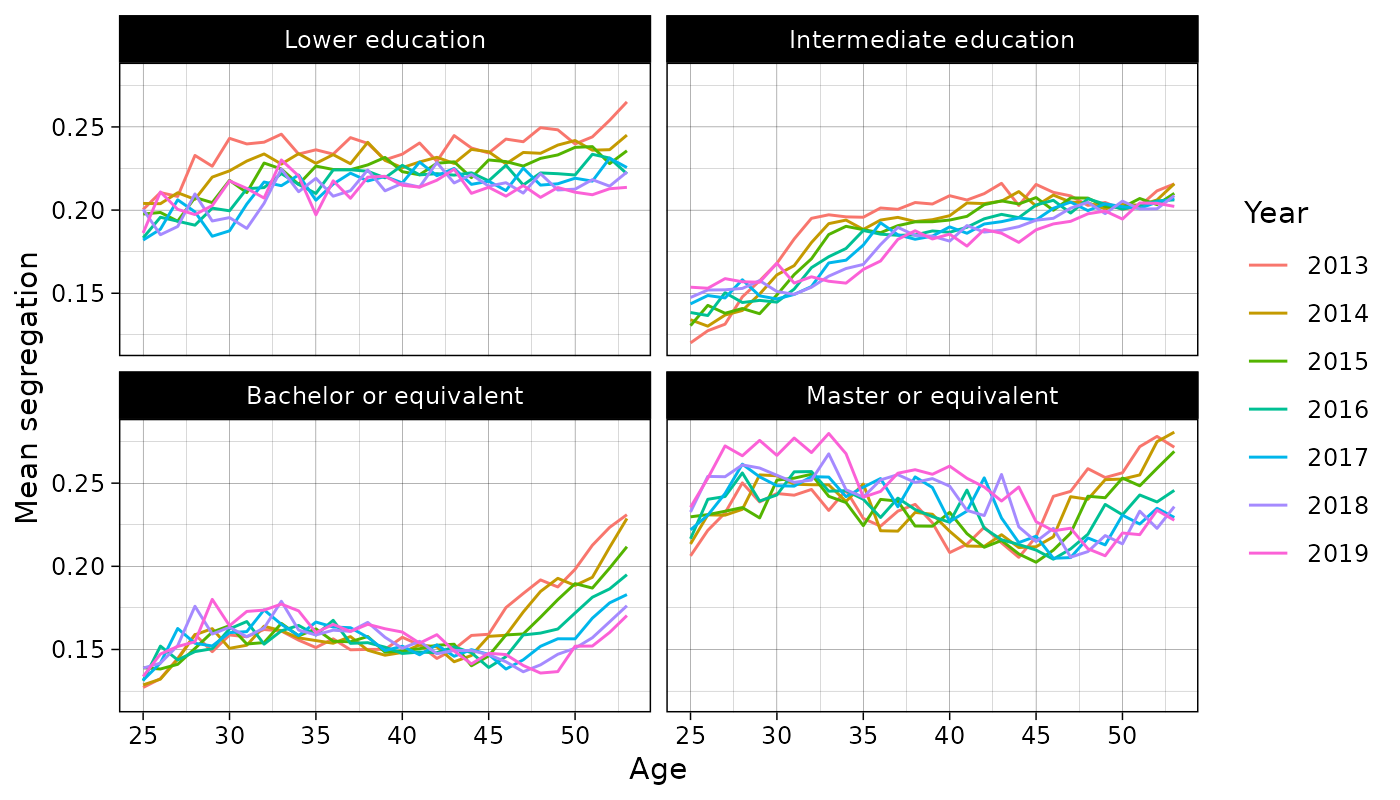
\includegraphics[width=\textwidth]{segregatie_naar_leeftijd.png}
  \caption{Educational segregation as a function of age for different years and education levels.}
  \label{fig:lft}
\end{figure}

\begin{figure}
  \centering
  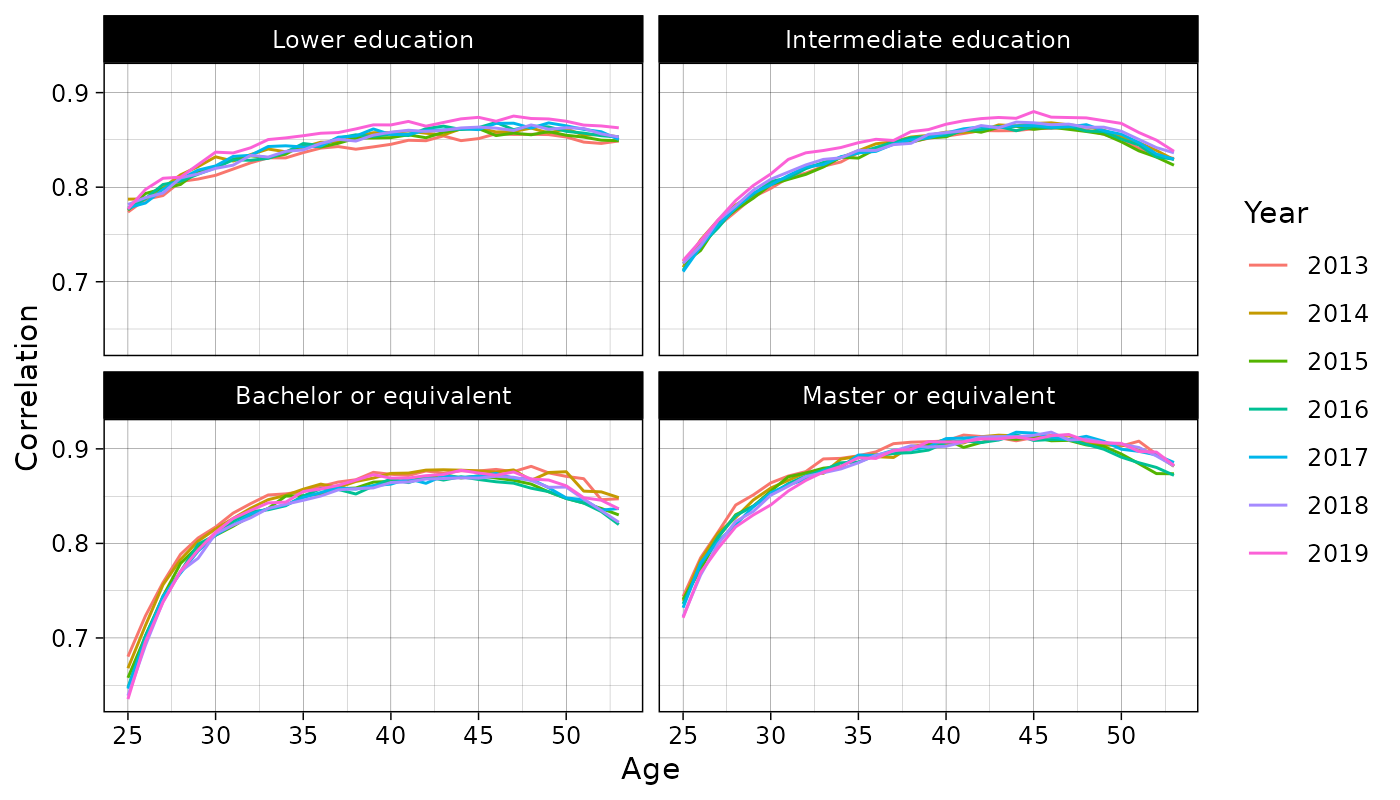
\includegraphics[width=\textwidth]{correlation.png}
  \caption{Correlation between individual educational segregation of year \textit{t} and year \textit{t}+1 as a function of age (measures in year $t$) for different years \textit{t} and different education levels.}
  \label{fig:cor}
\end{figure}


\begin{figure}
  \centering
  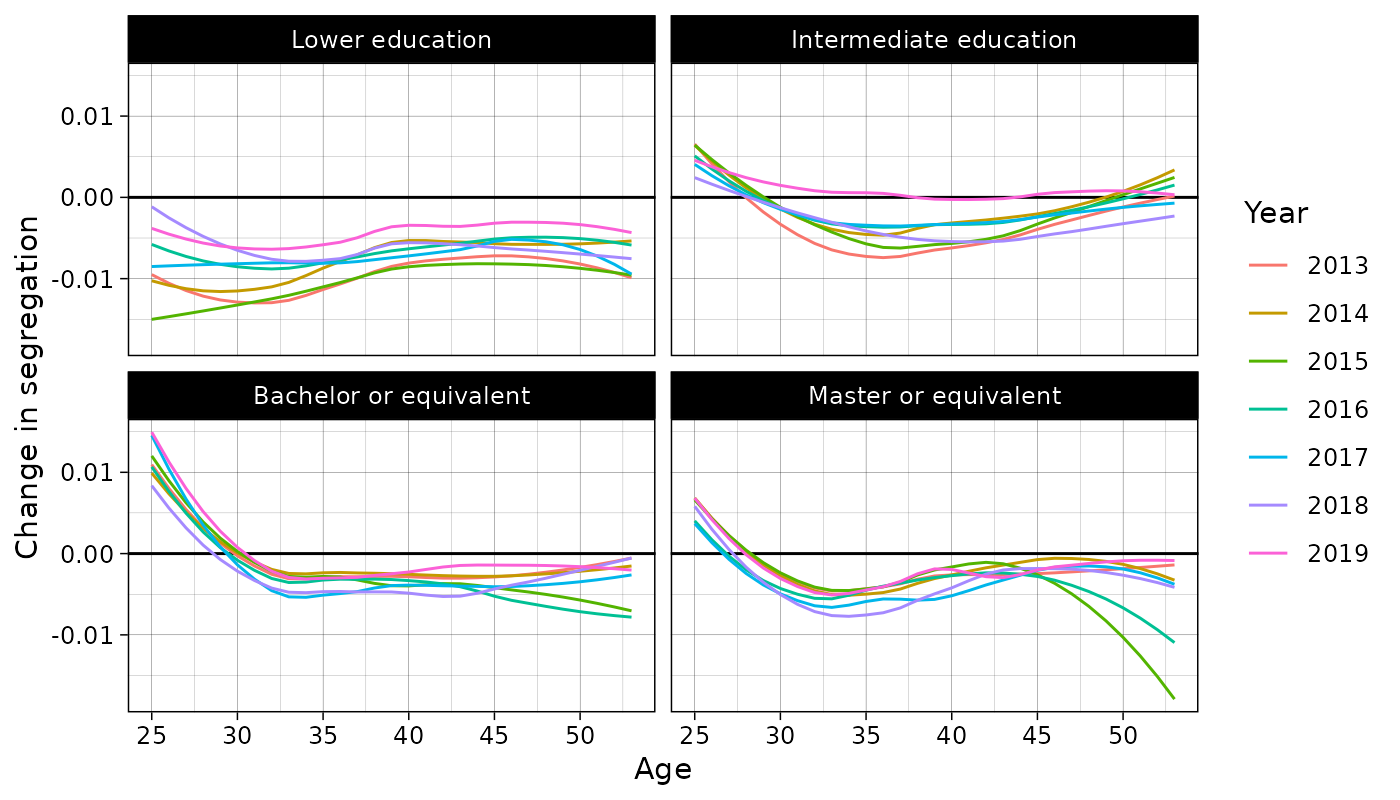
\includegraphics[width=\textwidth]{segregatie_ontwikkeling_leeftijd.png}
  \caption{Smoothed development of educational segregation between year \textit{t} and year \textit{t}+1 as a function of age (measures in year $t$) for different years \textit{t} and different education levels.}
  \label{fig:ontw}
\end{figure}




\end{document} 
